\documentclass[journal=jpcbfk]{achemso}

\usepackage[version=3]{mhchem}
\usepackage[T1]{fontenc}
\newcommand*\mycommand[1]{\texttt{\emph{#1}}}
%\newcommand{\todo}[1]{\textcolor{red}{#1}}
\usepackage[obeyFinal]{easy-todo}
\usepackage{rotating}
\usepackage{upgreek}				
\usepackage{xcolor}
\usepackage{booktabs}
\usepackage{multirow}
\usepackage{lmodern}
\usepackage{microtype}
\usepackage{xr-hyper}
\usepackage{soul} % for highlights with \hl{} 
\usepackage{hyperref} % to make TOC titles clickable
\hypersetup{
    colorlinks=true, %set true if you want colored links
    linktoc=all,     %set to all if you want both sections and subsections linked
    linkcolor=black,  %choose some color if you want links to stand out
    citecolor=black,
    filecolor=black,
    urlcolor=black
}

\makeatletter
\newcommand*{\addFileDependency}[1]{% argument=file name and extension
  \typeout{(#1)}
  \@addtofilelist{#1}
  \IfFileExists{#1}{}{\typeout{No file #1.}}
}
\makeatother

\newcommand*{\myexternaldocument}[1]{%
    \externaldocument{#1}%
    \addFileDependency{#1.tex}%
    \addFileDependency{#1.aux}%
}

\myexternaldocument{manuscriptPGPE}



\author{\scriptsize Am{\'e}lie Bacle}
\affiliation{Laboratoire Coop\'{e}ratif "Lipotoxicity and Channelopathies - ConicMeds", Universit\'{e} de Poitiers, 1 rue Georges Bonnet, 86000 Poitiers, France }

\author{\scriptsize Pavel Buslaev}
\affiliation{\tiny Nanoscience Center and Department of Chemistry, University of Jyväskylä, P.O. Box 35, 40014 Jyväskylä, Finland}
\affiliation{Research Center for Molecular Mechanisms of Aging and Age-related Diseases, Moscow Institute of Physics and Technology, 141701 Dolgoprudny, Russia}

\author{Rebeca Garc{\'i}a Fandi{\~n}o}
\affiliation{Center for Research in Biological Chemistry and Molecular Materials (CiQUS), Universidade de Santiago de Compostela, E-15782 Santiago de Compostela, Spain}
\affiliation{CIQUP, Centro de Investigação em Química, Departamento de Química e Bioquímica, Faculdade de Ciências, Universidade do Porto, Porto, Portugal}

\author{Fernando Favela-Rosales}
\affiliation[Tecnol\'{o}gico Nacional de M\'{e}xico]{Departamento de Ciencias B\'{a}sicas, Tecnol\'{o}gico Nacional de M\'{e}xico, ITS Zacatecas Occidente, M\'{e}xico}

\author{Tiago Ferreira}
\affiliation{Halle, Germany}

\author{Patrick F.J. Fuchs}
\affiliation{Sorbonne Universit\'{e}, Ecole Normale Sup\'{e}rieure, PSL University, CNRS, Laboratoire des Biomol\'{e}cules (LBM), 75005 Paris, France}
\alsoaffiliation{Universit\'{e} de Paris, UFR Sciences du Vivant, 75013, Paris, France}

\author{Ivan Gushchin}
\affiliation{Research Center for Molecular Mechanisms of Aging and Age-related Diseases, Moscow Institute of Physics and Technology, 141701 Dolgoprudny, Russia}

\author{Matti Javanainen}
\affiliation[Czech Academy of Sciences]{Institute of Organic Chemistry and Biochemistry of the 
Czech Academy of Sciences, Flemingovo n\'{a}m. 542/2, CZ-16610 Prague 6, Czech Republic}

\author{Anne M. Kiirikki}
\affiliation{Institute of Biotechnology, University of Helsinki}

\author{Jesper J. Madsen}
\affiliation[University of Chicago]{Department of Chemistry, The University of Chicago, Chicago, Illinois, United States of America}
\alsoaffiliation[University of South Florida]{Global and Planetary Health, College of Public Health, University of South Florida, Tampa, Florida, United States of America}

\author{Josef Melcr}
\affiliation[Czech Academy of Sciences]{Institute of Organic Chemistry and Biochemistry of the 
Czech Academy of Sciences, Flemingovo n\'{a}m. 542/2, CZ-16610 Prague 6, Czech Republic}
\alsoaffiliation{Groningen Biomolecular Sciences and Biotechnology Institute 
and The Zernike Institute for Advanced Materials, 
University of Groningen, 9747 AG Groningen, The Netherlands}

\author{Paula Milán Rodríguez}
\affiliation{Sorbonne Université, Ecole Normale Supérieure, PSL University, CNRS, Laboratoire des Biomolécules (LBM), 75005 Paris, France}

\author{Markus S. Miettinen}
% \affiliation[Max Planck Institute of Colloids and Interfaces]{Department of Theory and Bio-Systems, Max Planck Institute of Colloids and Interfaces, 14424 Potsdam, Germany}
\affiliation{Department of Theory and Bio-Systems, Max Planck Institute of Colloids and Interfaces, 14424 Potsdam, Germany}

\author{O. H. Samuli Ollila}
\email{samuli.ollila@helsinki.fi}
\affiliation{Institute of Biotechnology, University of Helsinki}

\author{Chris G. Papadopoulos}
\affiliation{Université Paris-Saclay, CEA, CNRS, Institute for Integrative Biology of the Cell (I2BC), 91198, Gif-sur-Yvette, France}


\author{Antonio Pe{\'o}n}
\affiliation[]{Spain}

\author{Thomas J. Piggot}
\affiliation[University of Southampton]{Chemistry, University of Southampton, Highfield, Southampton SO17 1BJ, United Kingdom}

\author{{\'A}ngel Pi{\~n}eiro}
\affiliation{Departamento de F{\'i}sica Aplicada, Facultade de F{\'i}sica, Universidade de Santiago de Compostela, E-15782 Santiago de Compostela, Spain}

\author{Salla I. Virtanen}
\affiliation{Institute of Biotechnology, University of Helsinki}



%\author{O. H. Samuli Ollila}
%\email{samuli.ollila@helsinki.fi}
%%\homepage[]{Your web page}
%\affiliation{Institute of Organic Chemistry and Biochemistry,
%Academy of Sciences of the Czech Republic, 
%Prague 6, Czech Republic}
%\affiliation{Institute of Biotechnology, University of Helsinki}


\SectionNumbersOn

\renewcommand{\thetable}{S\arabic{table}}%
\renewcommand{\thefigure}{S\arabic{figure}}%
\renewcommand{\thesection}{S\arabic{section}}%
\renewcommand{\thepage}{S\arabic{page}}%

\title{ Supporting Information:\\Conformational plasticity of phospholipid headgroups in simulations and experiments}

\begin{document}
\tableofcontents{}


\clearpage
\section{R-PDLF and SDROSS experiments}

\begin{figure}[]
%  \centering
  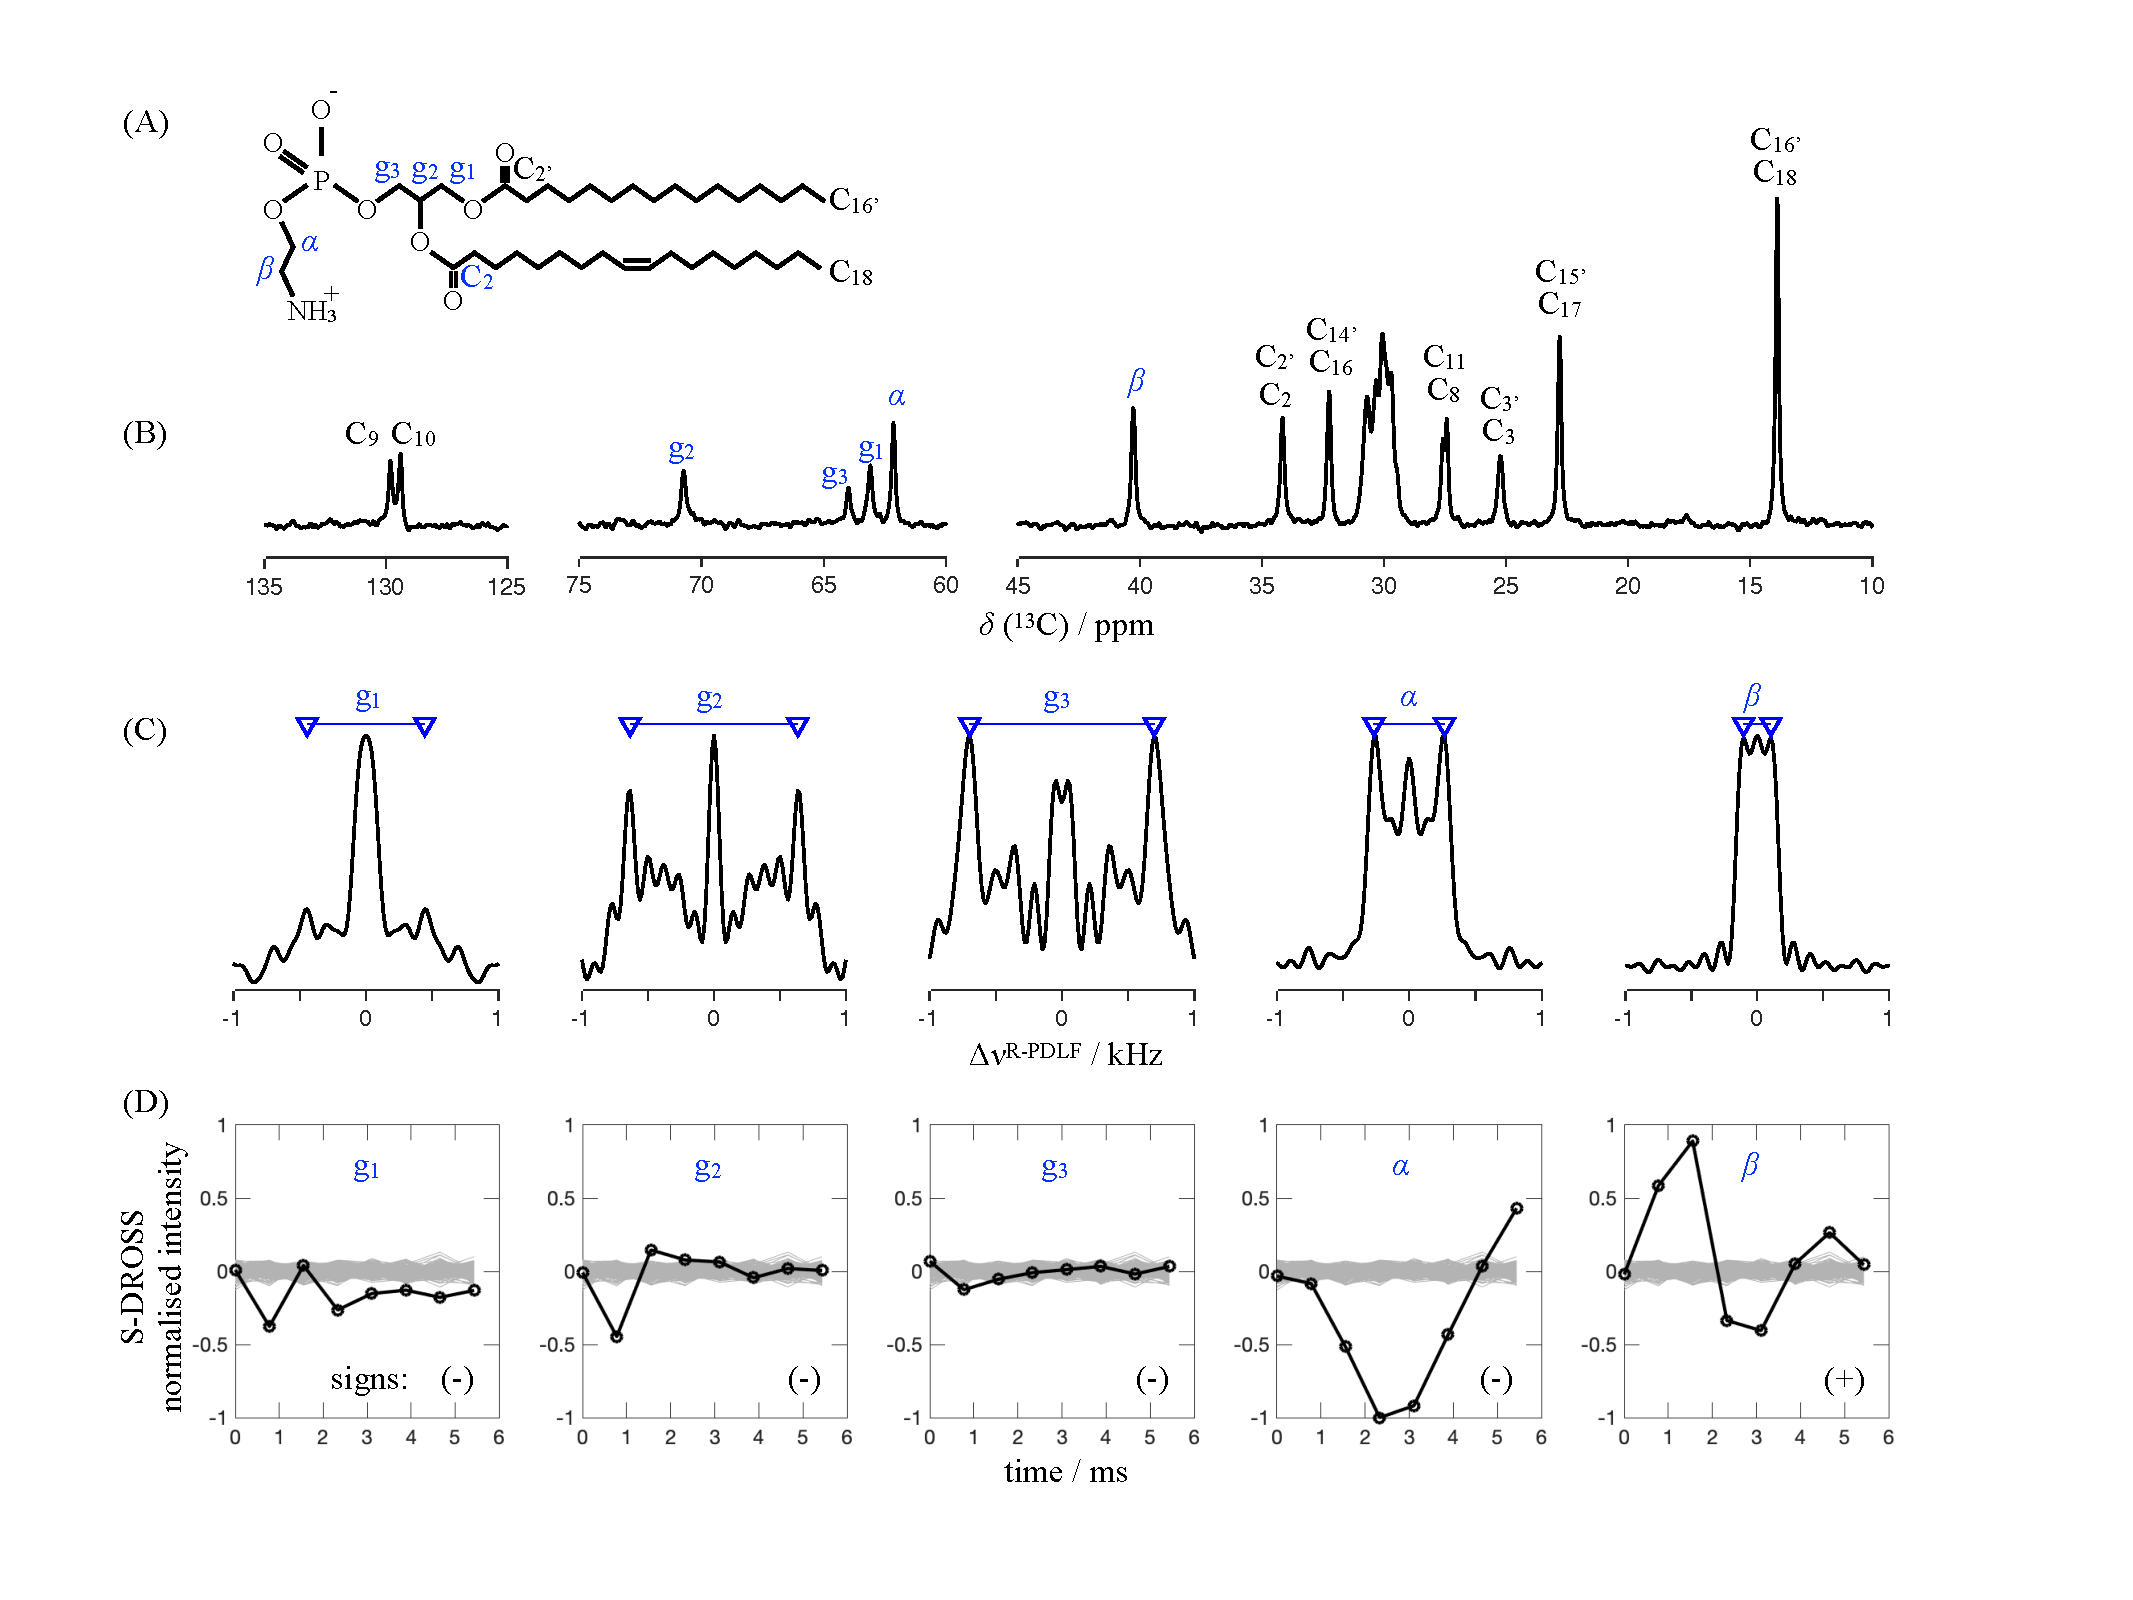
\includegraphics[width=0.9\textwidth]{./Figs/POPE_SI.pdf}
  \caption{\label{POPEspectra}
    Solid-state NMR spectroscopy for determining the C--H bond order parameters, $S_{\rm{CH}}$, in the POPE headgroup and glycerol backbone. (A) Chemical structure of POPE showing the labels used to identify different carbons.
    (B) Refocused INEPT $^{13}$C spectrum of POPE MLVs. 
    (C) Headgroup and glycerol backbone R-PDLF dipolar slices. The arrows indicate the splittings used to determine the C--H bond order parameters by using  $|S_{\rm{CH}}|=\Delta\nu/(0.315 \times d_{\rm{CH}})$. The rigid coupling $d_{\rm{CH}}$ used was 22 kHz.
    (D) Experimental S-DROSS curves giving signs of the order parameters measured.  Grey lines are a set of slices taken from a region of the spectrum without peaks, i.e. grey lines are noise profiles, to highlight the signal-to-noise ratio of the measured modulations.}
\end{figure}

\begin{figure}[]
%  \centering
  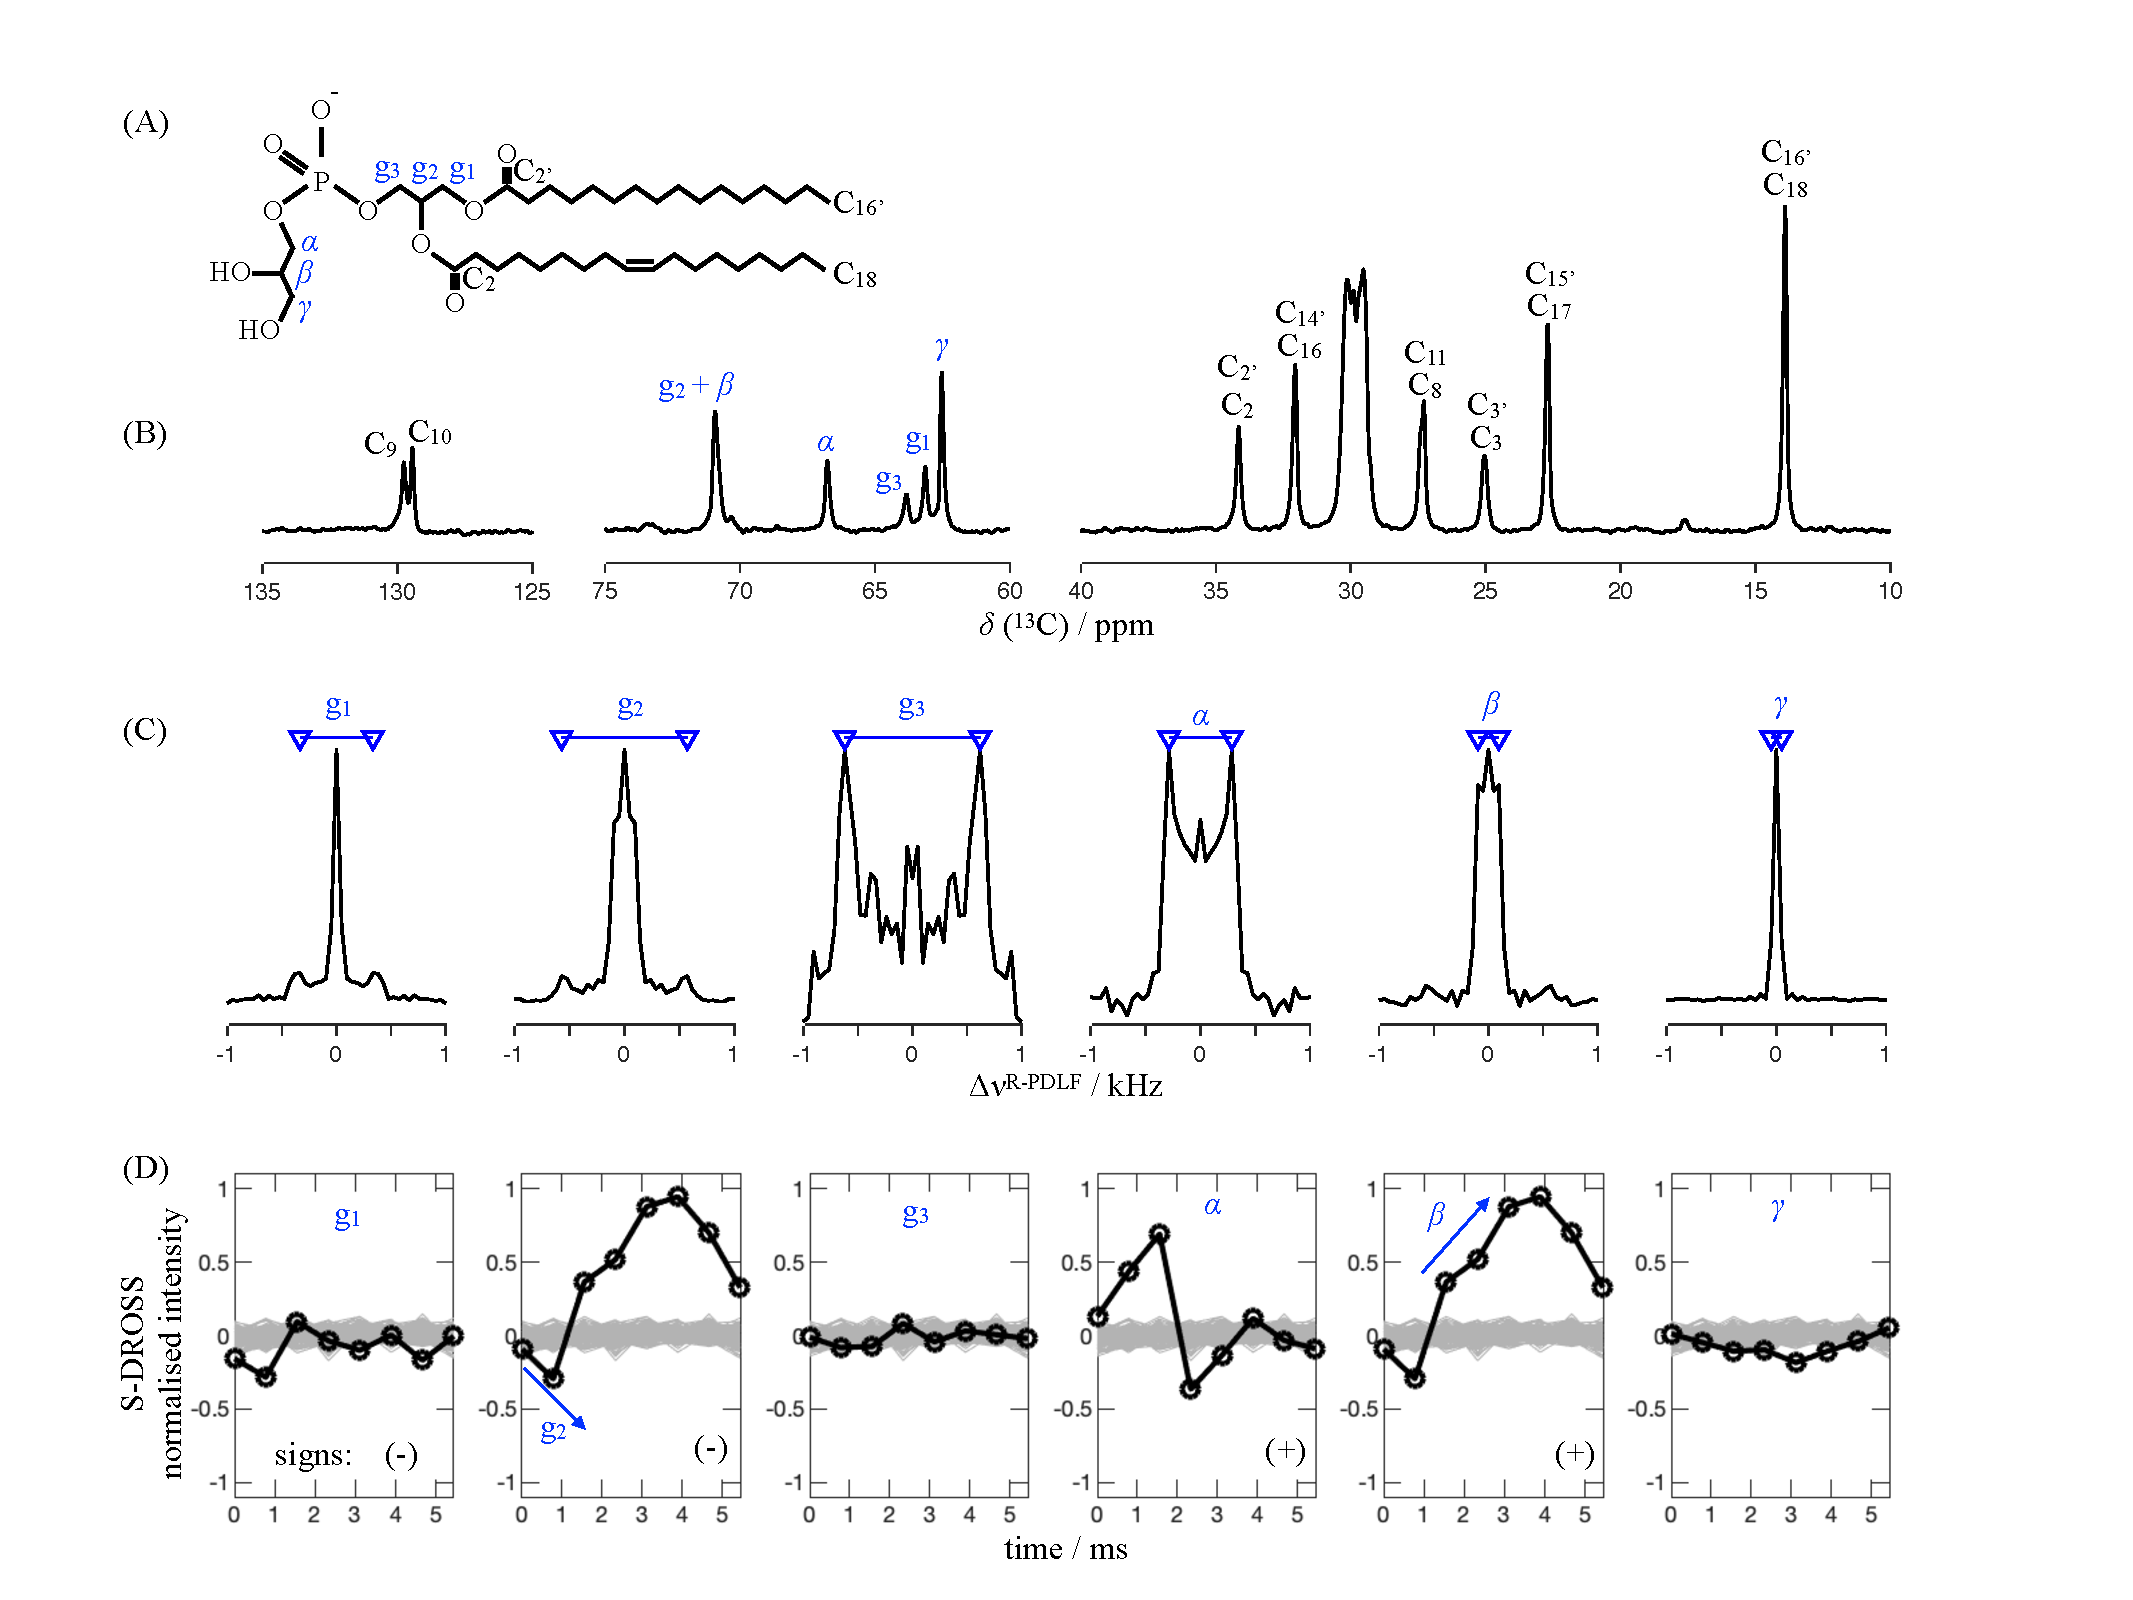
\includegraphics[width=\textwidth]{./Figs/POPG_SI.pdf}
  \caption{\label{POPGspectra}
    Solid-state NMR spectroscopy for determining the C--H bond order parameters, $S_{\rm{CH}}$, in the POPG headgroup and glycerol backbone. (A) Chemical structure of POPG showing the labels used to identify different carbons.
    (B) Refocused INEPT $^{13}$C spectrum of POPG MLVs.
    (C) Headgroup and glycerol backbone R-PDLF dipolar slices. The arrows indicate the splittings used to determine the C--H bond order parameters by using  $|S_{\rm{CH}}|=\Delta\nu/(0.315 \times d_{\rm{CH}})$. The rigid coupling $d_{\rm{CH}}$ used was 22 kHz.
    (D) Experimental S-DROSS curves giving signs of the order parameters measured.  Note that the S-DROSS modulation for $g_3$ is very close to the noise level. In this case, we have confirmed that the order parameter sign of $g_3$ was negative by performing a measurement with less points in the indirect dimension, more scans and using a higher MAS frequency of 8 kHz (not shown). 
  }
\end{figure}


\clearpage
\section{Lipid ligand names in PDB used in the analysis of conformations of protein-bound lipids}
{\bf PC:} PLC, PX4, 6PL, LIO, HGX, PC7, PC8, P1O, 6O8, XP5, EGY, PLD, SBM, HXG, and PCW \\
{\bf PE:} 8PE, PTY, 3PE, PEH, PEF, 6OE, 6O9, 9PE, PEV, 46E, SBJ, L9Q, PEK, EPH, ZPE, 9TL, 9Y0, 6OU, LOP, and PEE \\
{\bf PG:} PGT, PGK, LHG, 44G, PGV, OZ2, D3D, PGW, DR9, P6L, PG8, H3T, and GOT \\
{\bf PS:} PSF, PS6, Q3G, P5S, D39, PS2, 17F, and 8SP.


\clearpage
\section{Evaluation of simulations against NMR experiments}
\subsection{Conformational ensembles of headgroup and glycerol backbone in PE and PG lipids}

The quality of PE and PG headgroup conformational ensembles in different simulations are evaluated against NMR experiments in figures \ref{HGorderParametersPE} and \ref{HGorderParametersPOPG} using C-H bond order parameters as in our previous studies for PC and PS lipids \cite{botan15,antila19}. Conclusions are the same for all lipids: None of the force fields correctly captures the lipid headgroup conformational ensembles, but CHARMM36 gives results closest to experiments. Most importantly for this work, the CHARMM36 captures the distinct headgroup order parameters for PG and PS lipids observed in NMR experiments (Figs. \ref{HGorderParameters} and \ref{structures} in the main text). 

It should be noted that the PG headgroup is biologically abundant R enantiomer in all simulations, while our $^{13}$C NMR experiments has a racemic mixture. Nevertheless, previous $^{2}$H NMR experiments comparing results between different enantiomers concluded that the structural differences between these are minor \cite{wohlgemuth80}.

%The poor performance of headgroup order parameters in Berger model can be probably explained by
%ring like structures seen in Fig. 6 in Ref. \citenum{mukhopadhyay04}, which is a typical feature
%for Berger based lipid force fields containing explicit hydrogen atoms in the head group \cite{zhao08,henin09,dahlberg10}.
%The poor performance of glycerol backbone of Slipids simulations is systemically observed also
%for other lipids in previous studies \cite{botan15,antila19}.
%\todo{Should we comment more the relative quality of different force fields and/or make the subjective force field ranking figures?
%https://github.com/NMRLipids/NMRlipidsIVPEandPG/issues/8}

\begin{figure}[]
  \centering
  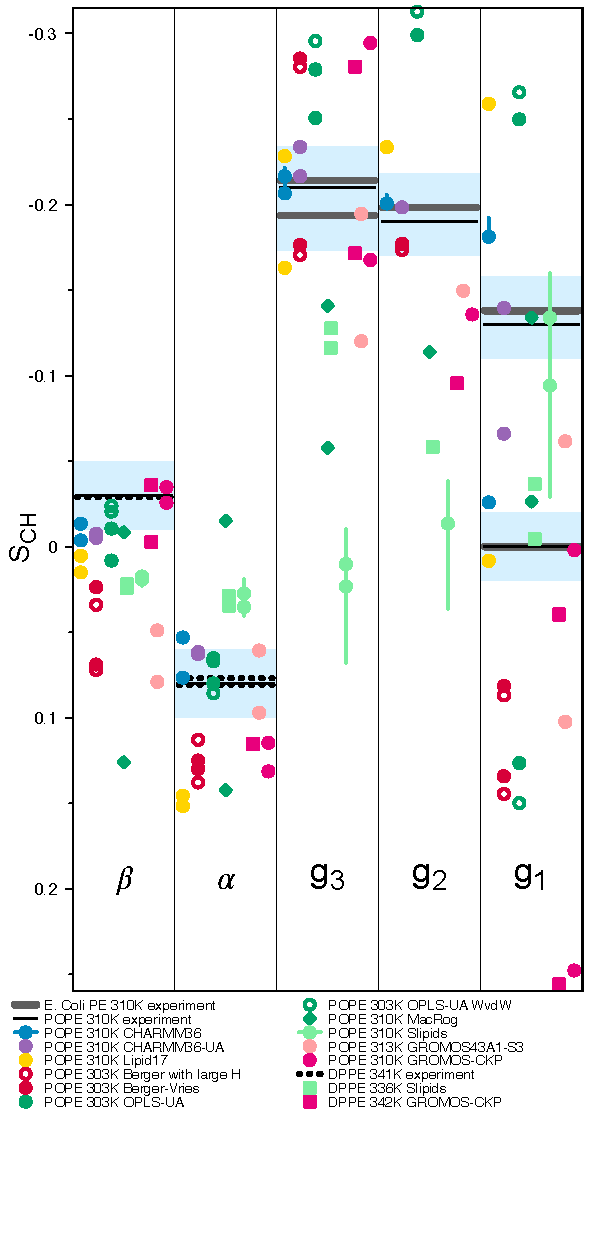
\includegraphics[width=9.0cm]{./Figs/HGorderparametersPE.pdf}
  \caption{\label{HGorderParametersPE}
    C--H bond order parameters, $S_{\rm CH}$, of the PE headgroup ($\beta$ and $\alpha$) and
    glycerol backbone (g$_3$, g$_2$, g$_1$) carbons from NMR experiments (horizontal lines;
    POPE and signs this work, DPPE from Ref.~\citenum{seelig76},
    {\it Escherichia coli} PE from Ref.~\citenum{gally81})
    and MD simulations with different force fields (symbols).
    The light blue areas span 0.04 units around the average of the extremal experimental values,
    in accordance with the expected quantitative accuracy of experiments~\cite{ollila16}.
    The vertical bars shown for most simulation values are not error bars,
    but demonstrate that for these systems we had at least two data sets;
    the ends of the bars mark the extreme values from the sets,
    the symbol marks the measurement-time-weighted average.
  }
\end{figure}

\begin{figure}[!h]
  \centering
  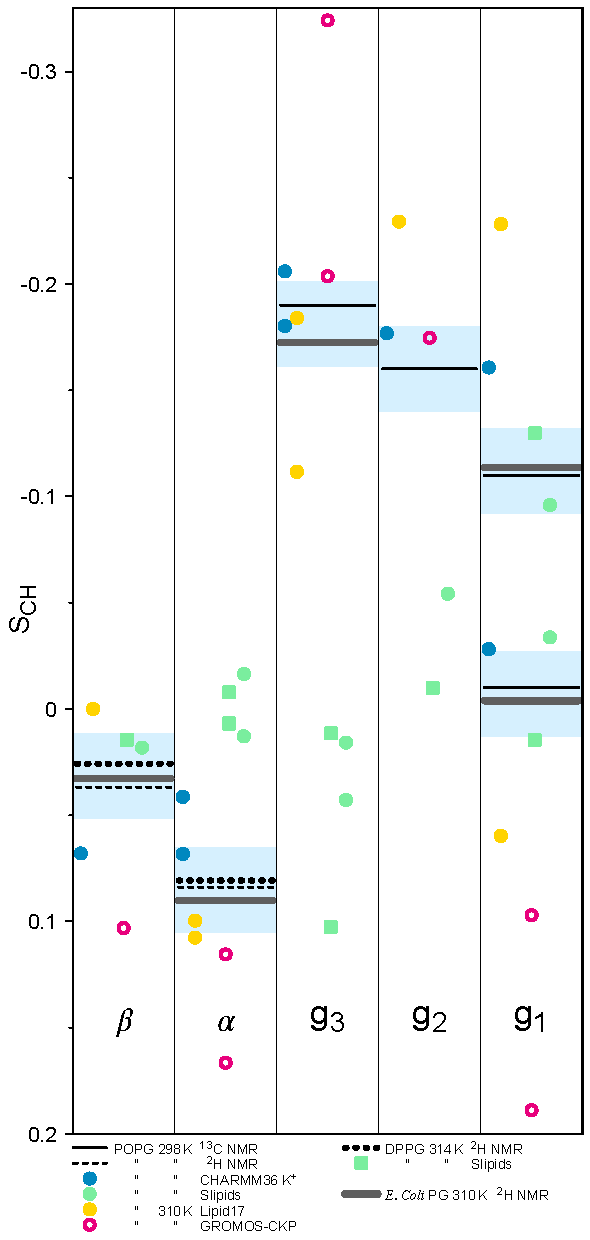
\includegraphics[width=9.0cm]{./Figs/HGorderparametersPG.pdf}
  \caption{\label{HGorderParametersPOPG}
    The headgroup and glycerol backbone order parameters of PG lipids
    from experiments (POPG and signs from this work and from Ref.~\citenum{borle85}, %contains 10mM of PIPES,
    DPPG with 100mM NaCl from Ref.~\citenum{wohlgemuth80},% contains 10mM PIPES and,
    and E.Coli PG results from Ref.~\citenum{gally81})
    and simulations with different force fields.
  }
\end{figure}

\clearpage

\subsection{PC headgroup in mixtures with PE or PG lipids}
\begin{figure*}[]
  \centering
  \includegraphics[width=16.0cm]{./Figs/HGorderparametersPCvsPEPG.eps}
  \caption{\label{HGorderparametersPCvsPEPG}
    Modulation of POPC headgroup order parameters with increasing amount of POPE (left) and POPG (right) in bilayer
    from experiments at 298 K \cite{scherer87,macdonald87} and simulations with different force fields
    (temperatures listed in tables \ref{systemsMIX} and \ref{systemsMIX2} are between 298-310 K).
    Signs are determined as discussed in Refs. \citenum{botan15,ollila16}.
  }
\end{figure*}

Headgroup order parameters of PC lipids are unchanged upon addition
of zwitterionic lipids or cholesterol in experiments, but increase
upon addition of negatively charged PG or PS lipids because
headgroup dipole tilts more parallel to the membrane plane after incorporation
of negative charges into the membrane~\cite{seelig87, scherer87,antila19}.
The response of PC headgroup order parameters to the addition of PE or PG lipids
from different simulations is compared with experiments in figure~\ref{HGorderparametersPCvsPEPG}.
None of the simulations reproduce neither the experimentally observed increase in PC headgroup order parameters
with increasing amount of PG nor the related tilting of the headgroup more parallel with the membrane.
Similar observations in our previous work for PS lipids were explained by the overestimated counterion
binding affinity that neutralizes the effect of added negative charge \cite{antila19}.
All simulations except Berger-OPLS predict tilting of P-N headgroup outwards from the membrane and
decrease of PC headgroup order parameters upon addition of PE lipids.
These results are not in line with experiments where the PC headgroup order parameters are not affected by zwitterionic lipids \cite{scherer87}.
The good performance of Berger-OPLS simulations is surprising here because
headgroup conformational ensemble is not very close to experiments in this model and
the response of headgroup order parameters
to cholesterol was significantly overestimated by the Berger/H{\"o}ltje force field in our previous work \cite{botan15}.

In conclusion, more accurate force fields are needed to correctly simulate the interactions between different headgroups.

\clearpage
\subsection{PG headgroup in mixtures with PC lipids}
Changes in other than PC lipid headgroup with changing membrane composition are less
extensively characterized in the literature.
The $\beta$-carbon order parameter in PG headgroup increases
mildly \cite{macdonald87} or is unchanged~\cite{borle85} upon increasing amount
of PC lipids (Fig. \ref{HGorderparametersPGvsPCchange}), but experimental data from
$\alpha$-carbon is not available. Also the tested force fields predict very small changes
for the $\beta$-carbon order parameter, while the P-N vector tilt and its response to the
increased amount of PC varies significantly between force fields in figure \ref{HGorderparametersPGvsPCchange}. 
Therefore, more experimental data and more accurate force fields are still required
to resolve the PG conformational ensembles in mixtures with other lipids.
\begin{figure}[]
  \centering
  \includegraphics[width=8.0cm]{./Figs/HGorderparametersPGvsPCchange.eps}
  \caption{\label{HGorderparametersPGvsPCchange}
    Modulation of PG lipid headgroup order parameters with the increasing amount of PC in lipid bilayer
    from experiments at 298 K \cite{borle85,macdonald87} and simulations with different force fields at 310 K.
  }
\end{figure}

\clearpage
\subsection{Calcium binding to POPC:POPG mixtures}

The changes of headgroup order parameters in POPC:POPG mixtures upon addition of CaCl$_2$ between different simulations
and experiments \cite{borle85,macdonald87} are compared in figures \ref{changesWITHCaClPG} (molar ratio 1:1) and \ref{changesWITHCaClPG1PC4} (molar ratio 4:1).
The results are in line with our previous studies:
most force fields overestimate the calcium binding \cite{catte16,antila19}, but CHARMM36 with the NBfix correction underestimates the binding affinity \cite{antila19}, and the implicit inclusion of electronic polarizability using the electronic continuum correction (ECC) improves the results \cite{melcr18,melcr20}.


\begin{figure*}[]
  \centering
  \includegraphics[width=18.0cm]{./Figs/CHANGESwithCaClPG1PC1.eps}
  \caption{\label{changesWITHCaClPG}
    Modulation of headgroup order parameters of POPC ({\it left}) and POPG ({\it right}) in POPC:POPG (1:1)
    mixture upon addition of CaCl$_2$ in 298 K temperature from experiments \cite{borle85,macdonald87} and simulations.
    The $\beta$-carbon order parameter of POPC (dashed line on top left) is not directly measured but
    calculated from empirical relation $\Delta S_{\beta}=0.43\Delta S_{\alpha}$ \cite{akutsu81}.
    The changes with respect to the systems without CaCl$_2$ are shown for other data than
    for the $\alpha$-carbon of POPG for which experimental order parameter is not available.
    Calsium density distributions are shown in figure \ref{CAdensPG}.
    %(right) The headgroup order parameters of PG from PC:PG mixtures as a function CaCl$_2$
    %concentration from experiments \cite{borle85} and CHARMM36 simulations.
  }
\end{figure*}


\begin{figure}[]
  \centering
  \includegraphics[width=8.0cm]{./Figs/CAdensPG1PC1.eps}
  \caption{\label{CAdensPG}
    Calcium ion density profiles along membrane normal from simulations of POPC:POPG (1:1) mixtures with different force fields.
    The changes in the order parameters upon addition of CaCl$_2$ are compared with experiments in figure \ref{changesWITHCaClPG}.
  }
\end{figure}

\begin{figure*}[]
  \centering
  \includegraphics[width=18.0cm]{./Figs/CHANGESwithCaClPG1PC4.eps}
  \caption{\label{changesWITHCaClPG1PC4}
    Modulation of headgroup order parameters of POPC ({\it left}) and POPG ({\it right}) in POPC:POPG (4:1)
    mixture upon addition of CaCl$_2$ in 298 K temperature from experiments \cite{macdonald87} and simulations.
    The changes with respect to the systems without CaCl$_2$ are shown for other data than
    for the $\alpha$-carbon of POPG for which experimental order parameter is not available.
  }
\end{figure*}

\begin{figure}[]
  \centering
  \includegraphics[width=8.0cm]{./Figs/CAdensPG1PC4.eps}
  \caption{\label{CAdensPG1PC4}
    Calcium ion density profiles along membrane normal from simulations of POPC:POPG (4:1) mixtures with different force fields.
  }
\end{figure}

\clearpage
\section{Dihedral angle distributions}
  

\subsection{Dihedral angles of PC, PE, PG and PS headgroups}

%The dihedral angle distributions are shown in Fig. \ref{DIHdists}
%and relative energies in Fig. \ref{structures} in the main text.

\begin{figure}[]
  \centering
  \includegraphics[width=7.0cm]{./Figs/DIHEDRALS.eps}
  \caption{\label{DIHdists}
    Heavy atom dihedral angle distributions from CHARMM36 simulations that correctly capture the order parameter differences between lipid headgroups.
  }
\end{figure}




\clearpage
\subsection{Changes in headgroup conformations upon addition of charged surfactants or CaCl$_2$}

\begin{figure}[]
  \centering
  \includegraphics[width=12.0cm]{./Figs/HGorderparametersPCvsSURFdihedrals.eps}
  \caption{\label{HGorderparametersPCvsSURFdihedrals}
    Changes in PC headgroup conformational ensembles upon increasing the amount of positive charge in bilayer,
    characterized by the heavy atom dihedral distributions, from CHARMM36 simulations.
  }
\end{figure}

\begin{figure}[]
  \centering
  \includegraphics[width=12.0cm]{./Figs/DIHEDRALSlipid17eccWITHCaClPOPC.eps}
  \caption{\label{DIHSwithCAlipid17eccPOPC}
    Changes in POPC lipid17ecc dihedrals with increasing amount of CaCl$_2$.
  }
\end{figure}

\begin{figure}[]
  \centering
   \includegraphics[width=12.0cm]{./Figs/DIHEDRALScharmm36WITHCaClPOPC.eps}
  \caption{\label{DIHSwithCAcharmm36POPC}
    Changes in POPC CHARMM36 dihedrals with increasing amount of CaCl$_2$.
  }
\end{figure}

\begin{figure}[]
  \centering
  \includegraphics[width=16.0cm]{./Figs/DIHEDRALSslipidsWITHCaClPOPG.eps}
  \caption{\label{DIHSwithCAslipidsPOPG}
    Changes in POPG Slipids dihedrals with increasing amount of CaCl$_2$.
  }
\end{figure}

\begin{figure}[]
  \centering
  \includegraphics[width=16.0cm]{./Figs/DIHEDRALSlipid17WITHCaClPOPG.eps}
  \caption{\label{DIHSwithCAlipid17POPG}
    Changes in POPG lipid17 dihedrals with increasing amount of CaCl$_2$.
  }
\end{figure}


\clearpage
\section{Simulated systems}

The simulated systems of pure PE and PG bilayers without additional ions
are listed in Tables~\ref{systemsPE} and \ref{systemsPG},
and lipid mixtures with additional ions in Tables~\ref{systemsMIX} and \ref{systemsMIX2}.
The simulations were analyzed using preliminary versions of the NMRlipids databank
(\url{www.nmrlipids.fi}, \url{github.com/NMRlipids/MATCH} and \url{https://github.com/NMRLipids/NMRlipidsIVPEandPG/tree/master/Data/Simulations})
and unique naming convention for lipid atoms (\url{http://nmrlipids.blogspot.com/2015/03/mapping-scheme-for-lipid-atom-names-for.html}),
which enable automatic analysis of simulations with different force fields with varying atom naming conventions.
The automatic analyses were implemented using MDAnalysis \cite{agrawal11,gowers16} and MDTraj \cite{mcgibbon15}
python libraries, and tools in the GROMACS sofware package \cite{gromacsMANUAL}.
All codes are available from the project's GitHub repository \cite{NMRlipidsIVbgit}.

The C--H bond order parameters were calculated directly
from the carbon and hydrogen positions using the definition
\begin{equation}
S_{\rm CH}=\frac{1}{2}\left\langle 3\cos^2\theta -1 \right\rangle,
\end{equation}
where $\theta$ is the angle between the C--H bond and the membrane normal
(taken to align with $z$, with bilayer periodicity in the $xy$-plane).
Angular brackets denote average over all sampled configurations.
The order parameters were first calculated averaging over time separately
for each lipid in the system. The average and
the standard error of the mean were then calculated over different lipids.
Code for all atom simulations is available in Ref.~\citenum{MATCHgit} (\texttt{scripts/calcOrderParameters.py}).
For united atom simulations, we first constructed trajectories including hydrogens with ideal geometry using either \texttt{buildH} program~\cite{buildH} or (\texttt{scratch/opAAUA\_prod.py}) in  Ref.~\citenum{MATCHgit}, and the order parameters were then calculated from these trajectories. This approach has been tested against trajectories with explicit hydrogens and the deviations in order parameters are small \cite{buildH,piggot17}.\\
%\todo{BuildH program is now cited with a direct link to the GitHub repo. I think that a release to Zenodo would be nice in the final publication.}\\



\begin{table*}[htb]
%
%\begin{sidewaystable*}[!p]
  \centering
  \caption{List of MD simulations with PE lipids.
    % The salt concentrations calculated as [salt]=N$_{\rm c} \times$[water]\,/\,N$_{\rm w}$, where [water]\,=\,55.5~M.
    % these correspond the concentrations reported in the experiments by Akutsu et al.~\cite{akutsu81}.
    % The lipid force fields named as in our previous work~\cite{botan15}.
  }\label{systemsPE}
  \begin{minipage}[t]{\textwidth}
  \resizebox{\columnwidth}{!}{
%    \begin{tabular}{l c c r r r r r r c c}
    \begin{tabular}{l c r r r r r c c}
      %\hline
      % some footnotes are not visible in typeset-MS (pdf)
      lipid 	& force field for lipids  %& NaCl (M) 
      		& \footnote{Number of lipid molecules}N$_{\rm l}$   &  \footnote{Number of water molecules}N$_{\rm w}$   %& \footnote{Number of additional cations}N$_{\rm c}$   
		& \footnote{Simulation temperature}T (K)  & \footnote{Total simulation time}t$_{{\rm sim}}$(ns) & \footnote{Time used for analysis}t$_{{\rm anal}}$ (ns) &   \footnote{Reference for simulation files}files\\
      \hline
      POPE & CHARMM36 \cite{klauda10}           %&0       
      		& 144	& 5760  %&0    
		& 310  & 500          & 400          & \citenum{charmm36POPEfiles} \\
      POPE & CHARMM36 \cite{klauda10}           %& 0      
      		& 500       & 25000 %& 0   
		&  310  & 500 & 100 & \citenum{POPEcharmm} \\
%   POPE	& CHARMM36 \cite{klauda10}           %& 0.11
%		& 500       & 25000 & 50  &  310  & 500 & 100 & \cite{POPEcharmm150mMNaCl} \\
      POPE	& CHARMM36-UA \cite{lee14}         %&0       
      		& 336	& 15254 %&0    
		& 310  & 2$\times$200 & 2$\times$100 & \citenum{charmm36uaPOPEfiles}  \\
      \hline
      DPPE	& Slipids \cite{jambeck12b}    %&0    
      		& 288 	& 9386  %&0    
		& 336  & 200 & 100 & \citenum{slipidsDPPEfiles}  \\
      POPE	& Slipids \cite{jambeck12b} %&0    
      		& 336	& ?     %&0    
		& 310  & 2$\times$200 &  2$\times$100 & \citenum{slipidsPOPEfiles}  \\
      POPE	& Slipids \cite{jambeck12b}            %& 0
		& 500 & 25000 %& 0   
		&  310  & 500 & 100 & \citenum{POPEslipids} \\
%      POPE  & Slipids / {\AA}qvist \cite{jambeck12b,aqvist90}  %& 0.11
%		& 500 & 25000 & 50  &  310  & 500 & 100 & \cite{POPEslipids150mMNaCl} \\
      \hline
      DPPE	& GROMOS-CKP    \cite{piggot11}      %&0
          	& 128	& 3655  %&0    
		& 342  & 2$\times$500 & 2$\times$400 & \citenum{gromosCKPdppe} \\
%      POPE  & GROMOS-CKP    \cite{??}      %&0
%    		& 128	& 3552  &0    & 313  & 2$\times$500 & 2$\times$400 & \cite{gromosCKPpope} \\
      POPE	& GROMOS-CKP    \cite{piggot11}      %&0
          	& 500	& 25000 %&0    
		& 310  & 500 & 100 & \citenum{gromosCKPpopeT310} \\
%      POPE  & GROMOS-CKP    \cite{??}      &0.11 & 500	& 25000 &50   & 310  & 500 & 100 & \cite{gromosCKPpopeT310150mMNaCl} \\
%      DOPE  & GROMOS-CKP    \cite{??}      &0    & 128	& 4789  &0    & 271  & 2$\times$500 & 2$\times$400 & \cite{gromosCKPdope} \\
      \hline
      POPE	& GROMOS 43A1-S3 \cite{chiu09}     %&0
          	& 128	& 3552     %&0    
		& 313  & 2$\times$200 & 2$\times$100 & \citenum{gromos43a1s3POPEfiles}  \\
      \hline
      POPE	& OPLS-UA/HG-H \cite{Ulmschneider09}   %&0    
      		& 128	& 3328     %&0    
		& 303  & 2$\times$200 & 2$\times$100 & \citenum{OPLSuaWvdWPOPEfiles} \\
      POPE	& OPLS-UA \cite{Ulmschneider09}            %&0
      		& 128	& 3328     %&0    
		& 303  & 2$\times$200 & 2$\times$100 & \citenum{OPLSuaPOPEfiles} \\
      \hline
      POPE	& OPLS-MacRog \cite{rog16}     %&0    
      		& 144	& 5760     %&0    
		& 310  & 500 & 350 & \citenum{MacRogPOPEfiles} \\
%   POPE	& OPLS-MacRog \cite{rog16}     &0    & 128	& 5120     &0    & 300  & 500 & 300 & \cite{MacRogPOPEfilesT300K} \\
      \hline
      POPE	& Berger-POPE-2004 \cite{devries04}       %&0    
      		& 128	& 3552  %&0    
		& 303  & 2$\times$200 & 2$\times$100 & \citenum{bergerPOPEfiles}  \\
      POPE	& Berger-POPE-2018 \cite{devries04}      %&0    
      		& 128	& 3552  %&0    
		& 303  & 2$\times$200 & 2$\times$100 & \citenum{berger2POPEfiles}  \\
%   DOPE  & Berger-POPE-2004 \cite{??}       &0    & 128	& 4789  &0    & 271  & 2$\times$200 & 2$\times$100 & \cite{bergerDOPEfiles}  \\
%   DOPE  & Berger-POPE-2018 \cite{??}      &0    & 128	& 4789  &0    & 271  & 2$\times$300 & 2$\times$100 & \cite{berger2DOPEfiles} \\ 
      \hline
      POPE	& Lipid17 \cite{gould18} %& 0      
      		& 500 & 25000 %& 0  
		&  310  & 500 & 100 & \citenum{POPElipid17} \\
%      POPE             & Lipid17 \cite{gould18} & 0.11   & 500 & 25000 & 50  &  310  & 500 & 100 & \cite{POPElipid17150mMNaCl} \\
    \end{tabular}
    }
  \end{minipage}
  %\todo{Which ion model is used in \cite{POPEcharmm150mMNaCl}?} \\
\end{table*}
%  \end{sidewaystable*} 

      \begin{table*}[htb]
  %\begin{sidewaystable*}[!p]
  \centering
  \caption{List of MD simulations with PG lipids.
    % The salt concentrations calculated as [salt]=N$_{\rm c} \times$[water]\,/\,N$_{\rm w}$, where [water]\,=\,55.5~M.
    % these correspond the concentrations reported in the experiments by Akutsu et al.~\cite{akutsu81}.
    % The lipid force fields named as in our previous work~\cite{botan15}.
  }\label{systemsPG}
  \begin{minipage}[t]{\textwidth}
  \resizebox{\columnwidth}{!}{
    \begin{tabular}{l c c r r r r r r c c}
      %\hline
      % some footnotes are not visible in typeset-MS (pdf)
      lipid/counter-ions & force field for lipids / ions &  \footnote{Number of lipid molecules with largest mole fraction}N$_{\rm l}$   &  \footnote{Number of water molecules}N$_{\rm w}$   & \footnote{Simulation temperature}T (K)  & \footnote{Total simulation time}t$_{{\rm sim}}$(ns) & \footnote{Time used for analysis}t$_{{\rm anal}}$ (ns) &   \footnote{Reference for simulation files}files\\
      \hline
      POPG/K$^+$  & CHARMM36 \cite{venable13}        & 118& 4110    & 298  & 100 & 100 & \citenum{CHARMM36popg}  \\
%      POPG             & CHARMM36 \cite{venable13}        & 0.11           & 500 & 25000 & 49  &  310  & 500 & 100 & \cite{POPGcharmm150mMNaCl} \\
      POPG             & CHARMM36 \cite{venable13}                & 500 & 25000  &  310  & 500 & 100 & \citenum{POPGcharmm} \\
      \hline
      POPG/Na$^+$  & Slipids / {\AA}qvist \cite{jambeck13,aqvist90}            & 288 	& 10664   & 298  & 250 & 100 & \citenum{slipidsPOPGfiles} \\
      DPPG/Na$^+$  & Slipids / {\AA}qvist \cite{jambeck13,aqvist90}           & 288 	& 11232   & 314  & 200 & 100 & \citenum{slipidsDPPGfiles} \\
      DPPG/Na$^+$  & Slipids / {\AA}qvist \cite{jambeck13,aqvist90}           & 288 	& 11232   & 298  & 400 & 100 & \citenum{slipidsDPPGfilesT298K} \\
      POPG         & Slipids / {\AA}qvist \cite{jambeck13,aqvist90}      & 500 & 25000  &  310  & 500 & 100 & \citenum{POPGslipids} \\
%      POPG         & Slipids / {\AA}qvist \cite{jambeck13,aqvist90}    & 0.11    & 500 & 25000 & 49  &  310  & 500 & 100 & \cite{POPGslipids150mMNaCl} \\
      \hline
      POPG             & LIPID17 / Dang \cite{gould18,smith94,dang06}     & 500 & 25000  &  310  & 500 & 100 & \citenum{POPGlipid17} \\
%      POPG             & LIPID17 \cite{gould18}         & 0.11           & 500 & 25000 & 49  &  310  & 500 & 100 & \cite{POPGlipid17150mMNaCl} \\
      \hline
      POPG             & GROMOS-CKP \cite{piggot11}         & 500 & 25000 &  310  & 500 & 100 & \citenum{POPGgromosCKP} \\
%      POPG             & GROMOS-CKP \cite{??}         & 0.11           & 500 & 25000 & 49 &  310  & 500 & 100 & \cite{POPGgromosCKP150mMNaCl} \\
    \end{tabular}
    }
  \end{minipage}
\end{table*}
% \end{sidewaystable*}


\begin{table*}[htb]
%  \begin{sidewaystable*}[!p]
  \centering
  \caption{List of MD simulations with PE and PG lipids mixed with PC.
    % The salt concentrations calculated as [salt]=N$_{\rm c} \times$[water]\,/\,N$_{\rm w}$, where [water]\,=\,55.5~M.
    % these correspond the concentrations reported in the experiments by Akutsu et al.~\cite{akutsu81}.
    % The lipid force fields named as in our previous work~\cite{botan15}.
  }\label{systemsMIX}
  \begin{minipage}[t]{\textwidth}
    \resizebox{\columnwidth}{!}{
    \begin{tabular}{l c c r r r r r r c c}
      %\hline
      % some footnotes are not visible in typeset-MS (pdf)
      lipid/counter-ions & force field for lipids / ions & CaCl$_2$\,(M) &  \footnote{Number of lipid molecules with largest mole fraction}N$_{\rm l}$   &  \footnote{Number of water molecules}N$_{\rm w}$   & \footnote{Number of additional cations}N$_{\rm c}$  & \footnote{Simulation temperature}T (K)  & \footnote{Total simulation time}t$_{{\rm sim}}$(ns) & \footnote{Time used for analysis}t$_{{\rm anal}}$ (ns) &   \footnote{Reference for simulation files}files\\
      \hline
%      POPC                   & CHARMM36 \cite{??}        & 0.11      & 0  & 500     & 25000 & 48  &  310  & 500 & 100 & \cite{POPCcharmm150mMNaCl301K}  \\
%      POPC:POPG (7:3)        & CHARMM36 \cite{??}        & 0.11      & 0  & 350     & ?     & ?   &  310  & 500 & 100 & \cite{POPC7POPG1charmm36NaCl}  \\
      POPC                   & CHARMM36 \cite{klauda10}            & 0  & 500     & 25000 & 0   &  310  & 500 & 100 & \cite{POPCcharmmT310K}  \\
      POPC:POPG (7:3)        & CHARMM36 \cite{klauda10,venable13}    & 0  & 350     & 25000 & 0   &  310  & 500 & 100 & \cite{POPC7POPG1charmm36}  \\
      POPC:POPG (1:1)        & CHARMM36 \cite{klauda10,venable13}     & 0  & 150:150 & 31500 & 0   &  298  & 500 & 400 & \cite{CHARMM36POPCPOPG5050} \\ 
      POPC:POPG (1:1)        & CHARMM36 \cite{klauda10,venable13}     & 0.1 & 150:150 & 31329 & 57 &  298  & 400 & 300 & \cite{CHARMM36POPCPOPG5050100mMCaCl} \\
      POPC:POPG (1:1)        & CHARMM36 \cite{klauda10,venable13}     & 1.08 & 150:150 & 29766 & 578  &  298  & 500 & 400 & \cite{CHARMM36POPCPOPG50501000mMCaCl} \\
      POPC:POPG (4:1)        & CHARMM36 \cite{klauda10,venable13}    & 0  & 350:88 & 26280 & 0  &  298  & 500 & 400 & \cite{CHARMM36POPCPOPG4010} \\
      POPC:POPG (4:1)        & CHARMM36 \cite{klauda10,venable13}    & 0.1 & 350:88 & 26280 & 47  &  298  & 500 & 400 & \cite{CHARMM36POPCPOPG4010100mMCaCl} \\
      POPC:POPG (4:1)        & CHARMM36 \cite{klauda10,venable13}    & 1.0 & 350:88 & 24927 & 451  &  298  & 500 & 400 & \cite{CHARMM36POPCPOPG40101000mMCaCl} \\
      \hline
      POPC             & CHARMM36 \cite{klauda10}        &0          & 256 & 8704 & 0  &  300  & 300 & 250 & \cite{POPCcharmm300K} \\
      POPC:POPE (1:1)  & CHARMM36 \cite{klauda10,venable13}         & 0  & 128 & 8704 & 0  &  300  & 300 & 250 & \cite{POPC1POPE1charmm36} \\
      \hline
      POPC             & OPLS-MacRog \cite{rog16}     &0           & 128 & 5120 & 0  &  300  & 500 & 300 & \cite{POPCmacrog300K} \\
      POPC:POPE (1:1)  & OPLS-MacRog \cite{rog16}     &0           & 128 & 5120 & 0  &  300  & 500 & 300 & \cite{POPC1POPE1macrogT300K} \\
      \hline
      POPC             & Slipid \cite{jambeck12b}     &0          & 512 & 23943 & 0  &  298  & 170 & 100 & \cite{POPCslipid298K} \\
      POPC:POPE (1:1)  & Slipid \cite{jambeck12b}     &0          & 128 & 5120  & 0  &  298  & 500 & 300 & \cite{POPC1POPE1slipidT298K} \\
     \hline
      POPC                   & GROMOS-CKP / ?? \cite{piggot12,??}  & 0  & 500     & 25000 & 0   &  310  & 500 & 100 & \cite{POPCgromosCKPT310K}  \\
      POPC:POPG (7:3)        & GROMOS-CKP / ?? \cite{piggot11,piggot12,??}  & 0  & 350:150 & 25000 & 0   &  310  & 500 & 100 & \cite{POPC7POPG3gromosCKPT310K} \\
     \hline
      POPC                   & Slipid \cite{jambeck12b}  & 0      & 500     & 25000 & 0   &  310  & 500 & 100 & \cite{POPCslipid301K}  \\
      POPC:POPG (7:3)        & Slipid / {\AA}qvist \cite{jambeck12b,aqvist90} & 0  & 350:150 & 25000 & 0   &  310  & 500 & 100 & \cite{slipidPOPC70POPG30T310K} \\
      POPC:POPG (1:1)        & Slipid / Dang \cite{jambeck12b,jambeck2012another,smith94,dang06} & 0  & 128:128 & 12800 & 0   &  298  & 500 & 400 & \cite{slipidPOPC50POPG50T298K} \\
      POPC:POPG (1:1)        & Slipid / Dang \cite{jambeck12b,jambeck2012another,smith94,dang06} & 0.1  & 128:128 & 12800 & 23  &  298  & 500 & 400 & \cite{slipidPOPC50POPG50T298K} \\
      POPC:POPG (1:1)        & Slipid / Dang \cite{jambeck12b,jambeck2012another,smith94,dang06} & 0.2  & 128:128 & 12800 & 46  &  298  & 1500 & 500 & \cite{slipidPOPC50POPG50T298K} \\
      POPC:POPG (1:1)        & Slipid / Dang \cite{jambeck12b,jambeck2012another,smith94,dang06} & 0.5  & 128:128 & 12800 & 115 &  298  & 1500 & 500 & \cite{slipidPOPC50POPG50T298K} \\
      POPC:POPG (1:1)        & Slipid / Dang \cite{jambeck12b,jambeck2012another,smith94,dang06} & 1.0  & 128:128 & 12800 & 230 &  298  & 1500 & 500 & \cite{slipidPOPC50POPG50T298K} \\
    \end{tabular}
    }
  \end{minipage}
    \todo{ion model for GROMOS-CKP?} \\ % TJP: Most likely standard GROMOS but not my simulations so I've left the ion reference
\end{table*}
%\end{sidewaystable*}

\begin{table*}
%  \begin{sidewaystable*}[!p]
  \centering
  \caption{List of MD simulations with PE and PG lipids mixed with PC.
    % The salt concentrations calculated as [salt]=N$_{\rm c} \times$[water]\,/\,N$_{\rm w}$, where [water]\,=\,55.5~M.
    % these correspond the concentrations reported in the experiments by Akutsu et al.~\cite{akutsu81}.
    % The lipid force fields named as in our previous work~\cite{botan15}.
  }\label{systemsMIX2}
  \begin{minipage}[t]{\textwidth}
    \resizebox{\columnwidth}{!}{
    \begin{tabular}{l c c r r r r r r c c}
      %\hline
      % some footnotes are not visible in typeset-MS (pdf)
      lipid/counter-ions & force field for lipids / ions & CaCl$_2$\,(M) &  \footnote{Number of lipid molecules with largest mole fraction}N$_{\rm l}$   &  \footnote{Number of water molecules}N$_{\rm w}$   & \footnote{Number of additional cations}N$_{\rm c}$  & \footnote{Simulation temperature}T (K)  & \footnote{Total simulation time}t$_{{\rm sim}}$(ns) & \footnote{Time used for analysis}t$_{{\rm anal}}$ (ns) &   \footnote{Reference for simulation files}files\\
      \hline
      POPC:POPG (4:1)        & Lipid17 / Dang \cite{gould18,smith94,dang06}       & 0  & 350:88 & 26265 & 0  &  298  & 400 & 350 & \cite{Lipid17POPCPOPG8020} \\
      POPC:POPG (4:1)        & Lipid17 / Dang \cite{gould18,smith94,dang06}    & 0.1& 350:88 & 26124 & 47 &  298  & 400 & 250 & \cite{Lipid17POPCPOPG8020100mMCaCl} \\
      POPC:POPG (4:1)        & Lipid17 / Dang \cite{gould18,smith94,dang06}    & 1.0& 350:88 & 24840 & 475 &  298  & 1200 & 200 & \cite{Lipid17POPCPOPG80201000mMCaCl} \\
      POPC:POPG (1:1)        & Lipid17 / Dang \cite{gould18,smith94,dang06}   & 0  & 150:150 & 31572 & 0  &  298  & 320 & 200 & \cite{Lipid17POPCPOPG5050} \\
      POPC:POPG (1:1)        & Lipid17 / Dang \cite{gould18,smith94,dang06}   & 0.1& 150:150 & 31401 & 57 &  298  & 718 & 198 & \cite{Lipid17POPCPOPG5050100mMCaCl} \\
      POPC:POPG (1:1)        & Lipid17 / Dang \cite{gould18,smith94,dang06}  & 1.0& 150:150 & 29865 & 569 &  298  & 720 & 200 & \cite{Lipid17POPCPOPG50501000mMCaCl} \\
      \hline
      POPC:POPG (4:1)        & Lipid17ecc / ECC-ions \cite{pluharova14,kohagen16,martinek18}     &0     & 350:88 & 26265 & 0  &  298  & 400 & 300 & \cite{Lipid17eccPOPCPOPG8020} \\
      POPC:POPG (4:1)        & Lipid17ecc / ECC-ions \cite{pluharova14,kohagen16,martinek18}     & 0.1& 350:88 & 26124 & 47 &  298  & 400 & 300 & \cite{Lipid17eccPOPCPOPG8020100mMCaCl} \\
      POPC:POPG (4:1)        & Lipid17ecc / ECC-ions \cite{pluharova14,kohagen16,martinek18}     & 1.0& 350:88 & 24840 & 475 &  298  & 400 & 300 & \cite{Lipid17eccPOPCPOPG80201000mMCaCl} \\
      POPC:POPG (1:1)        & Lipid17ecc / ECC-ions \cite{pluharova14,kohagen16,martinek18}     & 0  & 150:150 & 31572 & 0  &  298  & 347.8 & 333 & \cite{Lipid17eccPOPCPOPG5050} \\
      POPC:POPG (1:1)        & Lipid17ecc / ECC-ions \cite{pluharova14,kohagen16,martinek18}     & 0.1& 150:150 & 29865 & 54 &  298  & 400 & 300 & \cite{Lipid17eccPOPCPOPG5050100mMCaCl} \\
      POPC:POPG (1:1)        & Lipid17ecc / ECC-ions \cite{pluharova14,kohagen16,martinek18}     & 1.0& 150:150 & 29865 & 569 &  298  & 600 & 400 & \cite{Lipid17eccPOPCPOPG50501000mMCaCl} \\
      \hline
      POPC             & Berger-POPC-?? \cite{??} \todoi{This is probable not plain berger, correct force filed should be described.}  & 0  & 256 & 10240 & 0  &  300  & 300 & 200 & \cite{POPCberger300K} \\
      POPC:POPE (1:1)  & Berger-POPE-04~\cite{devries04}  & 0  & 128 & 11008 & 0  &  300  & 300 & 200 & \cite{POPC1POPE1berger} \\
      %POPC:DOPE (1:1)  & Berger \cite{??}  \todoi{This is probable not plain berger, correct force filed should be described.} &0          & 0  & 128 & 10240 & 0  &  300  & 300 & 200 & \cite{POPC1DOPE1berger} \\
    % \hline
    %  DOPC             & Berger \cite{??}  \todoi{This is probable not plain berger, correct force filed should be described.} &0          & 0  & 256 & 11008 & 0  &  300  & 300 & 200 & \cite{DOPCberger300K} \\
      %DOPC:DOPE (1:1)  & Berger \cite{??}   \todoi{This is probable not plain berger, correct force filed should be described.}  &0          & 0  & 128 & 11008 & 0  &  300  & 300 & 200 & \cite{DOPC1DOPE1berger} \\
    \end{tabular}
    }
  \end{minipage}
  \todo{Citation and description for Berger-POPC-?? model?} \\
\end{table*}
%\end{sidewaystable*}

\clearpage

\subsection{CHARMM36}

\noindent {\it POPE} A lipid bilayer, consisting of a total of 144 POPE molecules, distributed equally between the two leaflets was set using CHARMM-GUI \cite{lee16}. The bilayer was solvated by 5760 water molecules (40 per lipid). The random initial configuration and topologies were generated using the CHARMM-GUI web portal, which provides  GROMACS-compatible simulation input files \cite{lee16}. CHARMM36 lipid parameters \cite{klauda10} were used for POPE, whereas the CHARMM-specific TIP3P water model \cite{jorgensen83} was used for water. The bilayer was simulated for 500~ns using GROMACS 2018.6 at 310~K.

The recommended simulation parameters for CHARMM36 force field in GROMACS were used \cite{lee16}. Namely, buffered Verlet lists were used to keep track of neighbouring atoms \cite{Pall13}. The Lennard-Jones potential was cut off at 1.2~nm with the forces switched to 0 between 1.0~nm and the cutoff value. The smooth PME algorithm \cite{darden93,essman95} was used to account for long-range electrostatics. The temperatures of the lipid and the solvent were separately coupled to a Nos\'{e}-Hoover thermostat \cite{nose84,hoover85} with a time constant of 1~ps and a target temperature of 310~K. The system was coupled to a semi-isotropic (isotropic on the membrane plane) Parrinello--Rahman barostat \cite{parrinello81} with a time constant of 5~ps, a reference pressure of 1~bar, and compressibility of 4.5$\times$10$^{-5}$~1/bar. The bonds with hydrogen atoms were constrained using p-LINCS \cite{hess07,hess97}. The simulation files are available at Ref.~\citenum{charmm36POPEfiles}.

%\noindent {\it POPE with additional NaCl} \todo{Simulation details by A. Peon.}

\noindent {\it POPG} Lipid bilayer containing 118 POPG molecules, 4110 TIP3P water molecules, and 118 potassium ions was build using CHARMM-GUI \cite{lee16}.
The system was simulated 100~ns, coupled to 298 K using Nose-Hoover~\cite{nose84,hoover85} thermostat and 1 bar with
semi-isotropic Parrinello-Rahman~\cite{parrinello81} pressure coupling.
The used default parameters and force field files from CHARMM-GUI were used.
The used files are available from \citenum{CHARMM36popg}.

\todo{Simulation details for larger simulation by A. Peon.}

%\noindent {\it POPG with additional NaCl} \todo{Simulation details by A. Peon.}

\noindent {\it POPC:POPE mixtures} 
A pure POPC system and a 50:50 POPC:POPE mixture were built and equilibrated using CHARMM-GUI~\cite{lee16}.
They contained 256 lipids (for the mixture 64 lipids per leaflet for each species) and 34 water molecules per lipid.
No ions were added.
The production simulations were run for 300 ns with a time step of 2 fs.
The first 50 ns were discarded for the analysis.
The simulations were run with the GROMACS 2016.4~\cite{abraham2015gromacs} version.
The v-rescale thermostat~\cite{bussi07} was used with a temperature of 300 K and a time constant of 1 ps; lipids and water were coupled separately to the heat bath.
Pressure was kept constant at 1 bar using a semi-isotropic Parrinello--Rahman barostat~\cite{parrinello81} with a time constant of 5.0 ps.
A real space cut-off of 1.2 nm was employed for electrostatic interactions while the long-range part was evaluated using the PME method~\cite{darden93,essman95}.
A force-based switching function was used to switch the Lennard-Jones forces to zero over a range of 1--1.2 nm.
All bonds with hydrogen atoms were constrained with the LINCS algorithm~\cite{hess07,hess97}.
Water molecules were kept rigid with the SETTLE algorithm~\cite{miyamoto92}.
The simulation files are available from Ref.~\citenum{POPCcharmm300K} (pure POPC) and~\citenum{POPC1POPE1charmm36} (POPC:POPE mixture).

\noindent {\it POPC:POPG 1:1 and POPC:POPG 4:1 mixtures with additional calcium} 
The initial structures were built with CHARMM-GUI Membrane Builder \cite{lee16}. The TIP3P water model was used to solvate the systems. The simulations were run for 400~ns with timestep 2~fs and the first 100~ns were discarded as equilibration time. The simulations were run with GROMACS version 2020.2~\cite{pall20}. The Nose-Hoover thermostat~\cite{nose84,hoover85} was used with temperature of 298~K and the time constant for temperature coupling was 1.0~ps. The semi-isotropic Parrinello-Rahman barostat~\cite{parrinello81} was used with reference pressure 1.0~bar and with a time constant of 5.0~ps with compressibility of 4.5e-5~bar$^{-1}$. Long range electrostatic interactions were calculated with the PME method. All bonds with hydrogen atoms were constrained with LINCS algorithm.
The simulation files are available from Refs.~\citenum{CHARMM36POPCPOPG5050,CHARMM36POPCPOPG5050100mMCaCl,CHARMM36POPCPOPG50501000mMCaCl,CHARMM36POPCPOPG4010,CHARMM36POPCPOPG4010100mMCaCl,CHARMM36POPCPOPG40101000mMCaCl}.


\noindent {\it POPC and POPC:POPG (7:3) mixture} \todo{Simulation details by A. Peon.}

\noindent {\it POPC and cationic surfactant (dihexadecyldimethylammonium) mixture}
Intial structures were taken from similar previously published \cite{melcr18} simulations with Amber lipid14 force field,
which are available from Ref. \citenum{POPClipid14T313K,POPClipid1410perCATsurfT313K,POPClipid1420perCATsurfT313K,POPClipid1430perCATsurfT313K,POPClipid1442perCATsurfT313K,POPClipid1450perCATsurfT313K}.
Default simulations parameters and force field files from CHARMM-GUI \cite{lee16} were used, except for dihexadecyldimethylammonium
for which the atom types and partial charges of Amber lipid14 parameters from previous work \cite{melcr18} were modified to correspond Charmm36
force field. 
Systems contained 50 POPC molecules, 3983 water molecules, and 12, 30, 44, or 88 dihexadecyldimethylammonium molecules.
Chloride ions were used as counterions for dihexadecyldimethylammonium.
Reference system without cationic surfactants contained 200 POPC and 9000 water molecules.
Systems were simulated 200 ns (the first 20 ns was discarded as an equilibration period)
using Gromacs 5 \cite{abraham2015gromacs} at the temperature of 313 K.
All simulation files are available from Refs. \citenum{charmmPOPC313K,CHARMM36cationicSURF}.

\subsection{CHARMM36-UA}

\noindent {\it POPE} Data is available at \cite{charmm36uaPOPEfiles}. CHARMM36-UA POPE simulations were performed for 200 ns using GROMACS version 5.0.6. A topology for POPE was constructed using the standard CHARMM36 all-atom PE head group combined with the original CHARMM36-UA lipid tail parameters \cite{lee14}. Simulations were performed using a hexagonal periodic box containing 336 POPE lipids. This membrane was constructed using a MARTINI force field \cite{marrink07} coarse-grained self-assembly simulation followed by reverse-mapping to an atomic resolution. Simulations were performed using standard CHARMM lipid simulation settings; further details are available at \cite{charmm36uaPOPEfiles}.

%\subsection{MacRog}

%\subsection{Lipid17}

\subsection{Slipids}
\noindent {\it POPE} Data is available at \cite{slipidsPOPEfiles}. Slipids POPE simulations were performed for 200 ns using GROMACS version 5.0.6. Simulations employed the original Slipids POPE parameters \cite{jambeck12b} and employed the same starting structure as the CHARMM36-UA POPE simulations. Slipids simulations employed standard AMBER force field cut-offs of 1.0 nm, previously validated for use with the Slipids force field \cite{piggot17}. Further simulation details are available at \cite{slipidsPOPEfiles}.

%\noindent {\it POPE with additional NaCl} \todo{Simulation details by A. Peon.
%  I have assumed that ion parameters are default Slipids, i.e., {\AA}qvist, please correct if this is not true.
%}

\noindent {\it DPPE with 288 lipids.} The starting structure for simulation
with 288 DPPE lipids and 9386 water molecules
was constructed with the MEMBRANE BUILDER website~\cite{ghahremanpour13}. The TIP3P~\cite{jorgensen83} water model was used to solvate the system.
Simulation was performed for 200~ns, and the last 100~ns were used for the analysis. Simulation was carried out within the NPT ensemble using the GROMACS 5.0.4 package~\cite{abraham2015gromacs}. Timestep of 2~fs was used with the leapfrog integrator. The Nos\'{e}--Hoover thermostat~\cite{nose84,hoover85} was used with reference temperature of 336~K and a relaxation time constant of 0.5~ps; lipids and water were coupled separately to the heat bath. Pressure was kept constant at 1.013~bar using a semi--isotropic Parrinello--Rahman
barostat~\cite{parrinello81} with a time constant of 10.0~ps. Long-range electrostatic interactions were calculated using the PME method~\cite{darden93,essman95}. A real space cut-off of 1.0~nm was employed with grid spacing of 0.12~nm in the reciprocal space. Lennard-Jones potentials were cut off at 1.4~nm, with a dispersion correction applied to both energy and pressure. All covalent bonds in lipids were constrained using the LINCS algorithm~\cite{hess97}, whereas water molecules were constrained using SETTLE~\cite{miyamoto92}. Twin-range cutoffs, 1.0~nm and 1.6~nm, were used for the neighbor lists with the long-range neighbor list updated every 10 steps.

\noindent {\it POPG with 288 lipids.} The starting structure for simulation
with 288 POPG lipids, 10664 water molecules and 288 Na ions
was constructed with the MEMBRANE BUILDER website~\cite{ghahremanpour13}. The TIP3P~\cite{jorgensen83} water model was used to solvate the system and Ions are described by the parameters derived by \AA qvist~\cite{aqvist90}.
Simulation was performed for 250~ns, and the last 100~ns were used for the analysis. Same simulation conditions as DPPE with reference temperature of 298~K.

%\noindent {\it POPG with additional NaCl} \todo{Simulation details by A. Peon.
%  I have assumed that ion parameters are default Slipids, i.e., {\AA}qvist, please correct if this is not true.}

\noindent {\it DPPG with 288 lipids.} The starting structure for simulation
with 288 DPPG lipids, 11232 water molecules and 288 Na ions
was constructed with the MEMBRANE BUILDER website~\cite{ghahremanpour13}. The TIP3P~\cite{jorgensen83} water model was used to solvate the system and Ions are described by the parameters derived by \AA qvist~\cite{aqvist90}. For the 298~K temperature, simulation was performed for 400~ns, and the last 100~ns were used for the analysis. For the 314~K temperature, simulation was performed for 200~ns, and the last 100~ns were used for the analysis. Same simulation conditions as DPPE for both temperatures.

\noindent{\it POPC:POPE mixture}
A POPC/POPE bilayer with its lipids distributed evenly among the leaflets was generated by from a pure POPC bilayer by removing and renaming atoms in the head group region. The bilayer contained a total of 100 POPC and 100 POPE lipids, and it was solvated by 45 water molecules per lipid (for a total of 9000 water molecules).
The Slipids force field \cite{jambeck12,jambeck12b,jambeck13} was used for lipids, and the TIP3P model \cite{jorgensen83} for water. A 300~ns-long simulation was performed using GROMACS 2019.4 \cite{abraham2015gromacs}. The simulation parameters were equal to those used for the POPC/POPG mixture with additional CaCl$_2$ (see below). 
The simulation data are available at Ref.~\citenum{POPC1POPE1slipidT298K}.

%\noindent {\it POPC:POPG mixture with additional NaCl} \todo{Simulation details by A. Peon.
%  I have assumed that ion parameters are default Slipids, i.e., {\AA}qvist, please correct if this is not true.}

\noindent {\it POPC:POPG mixture with additional CaCl$_2$} 
A lipid bilayer consisting of a total of 256 lipids (128 POPC + 128 POPG) spread equally between the two leaflets was generated using CHARMM-GUI \cite{lee16}. The membrane was solvated by 50 water molecules per lipid (a total of 12800), and 128 Na$^{+}$ counter ions for the POPG charges. The initial random configuration was equilibrated using the CHARMM-GUI protocol and using the CHARMM36 force field \cite{klauda10}. Next, additional ions were added to obtain initial CaCl$_2$ concentrations of 0, 100, 200, 500, or 1000~mM (0/0, 23/46, 46/92, 115/230, 230/460 Ca$^{2+}$/Cl$^{-}$ ions) The systems were energy-minimized and equilibrated using the Slipids force field \cite{jambeck12,jambeck12b,jambeck13} before production simulations at 298~K. The ion parameters by \citeauthor{dang06} were used \cite{dang06}.

The neighbour lists with a cutoff of 1.0~nm were updated every 10 simulation steps. The smooth PME algorithm was used to calculate long-range electrostatics \cite{darden93,essman95}. The Lennard-Jones potential was cut off at 1.0~nm, and the dispersion corrections \cite{shirts07} were applied to energy and pressure. The stochastic velocity rescaling thermostat \cite{bussi07} with a time constant of 0.5~ps and a target temperature of 298~K was applied separately to lipids and the solvent. A constant pressure of 1~bar was maintained by a Parrinello--Rahman barostat \cite{parrinello81} with a time constant of 10~ps and compressibility of 4.5$\times$10$^{-5}$~1/bar. The pressure coupling was performed semi-isotropically with the two simulation box vectors aligned along the membrane plane considered isotropic. All bonds were constrained using the p-LINCS algorithm \cite{hess97,hess07}.

The systems simulated for 1500~ns (CaCl$_2$-containing systems) or 500~ns (systems without CaCl$_2$). The simulations were performed using GROMACS 2019.4 \cite{abraham2015gromacs}, and the simulation files are available at Ref.~\citenum{slipidPOPC50POPG50T298K}.

\subsection{Berger}

Following the earlier convention in the NMRlipids Project~\cite{botan15}, 
for the Berger-based models we use the following naming convention: 
Berger - \{{\it molecule name}\} - \{{\it year when model published first time}\} \{{\it citation}\}.
%The reason is that there are several different molecular topologies which are using the non-bonded parameters originally
%developed by Berger et al.~\cite{berger97}. Thus the common factor in the Berger based models are the non-bonded parameters,
%while the molecule specific parameters might somewhat vary. However, the majority of the molecular level topologies are 
%relying (especially for the glycerol backbone and headgroup) on the parameters originally introduced by Marrink et al.~\cite{marrink98}.

\noindent {\it POPE} Data are available at Ref.~\citenum{bergerPOPEfiles} for Berger-POPE-2004~\cite{devries04} and at Ref.~\citenum{berger2POPEfiles} for Berger-POPE-2018~\cite{berger2POPEfiles}. Simulations of POPE membranes using the Berger force field employed two variants of the Berger force field for PE lipids. The first (Berger-POPE-2004) used the de Vries modifications which includes additional repulsive Lennard-Jones interactions on the ethanolamine hydrogen atoms. The second (Berger-POPE-2018) used this same approach but doubled the repulsive strength employed for the hydrogen atom van der Waals interactions. The latter variant results in more disorder within the membrane and a closer agreement with experimental properties such as the area per lipid of POPE. POPE simulations were performed for 200 ns using GROMACS 5.0.6 and employed a POPE membrane with 64 lipids per leaflet taken from a published GROMOS-CKP POPE membrane \cite{piggot11}. Simulations used a 1.0 nm cut-off for both electrostatic and van der Waals interactions with PME and a dispersion correction doe the energy and pressure employed respectively. Further simulation details can be found at Ref.~\citenum{bergerPOPEfiles} and at Ref.~\citenum{berger2POPEfiles}.

%\noindent {\it DOPE} Data is available at \cite{bergerDOPEfiles,berger2DOPEfiles}. \todo{Simulation details by  T. Piggot.}

\noindent {\it POPC:POPE mixtures} 
Two systems were simulated using the Berger force field~\cite{Berger97}, pure POPC and a mixture 50:50 POPC:POPE. For POPE, we additionnally used the de Vries modification implementing a repulsion of the hydrogen atoms located on the amino group of ethanolamine~\cite{devries04}.
Starting from a PDB file of a pure POPC system with Berger atom names, a 50:50 POPC:POPE mixture was built by mutating randomly methyl groups to hydrogens (POPC -> POPE). Each system contained 256 lipids (for the mixture 64 lipids per leaflet for each species) and about 40 water molecules per lipid. No ions were added. Both systems were minimized and equilibrated. The production simulations were run for 300 ns with a time step of 2 fs. The first 100 ns were discarded for the analysis. The simulations were run with GROMACS 4.5.3~\cite{pronk13} version. The v-rescale thermostat~\cite{bussi07} was used with a temperature of 300 K and a time constant of 0.1 ps; lipids and water were coupled separately to the heat bath. Pressure was kept constant at 1 bar using a semi–isotropic Parrinello–Rahman barostat~\cite{parrinello81} with a time constant of 4.0 ps. A real space cut-off of 1.0 nm was employed for van der Waals and electrostatic interactions. The long-range part of electrostatic interactions was evaluated using the PME method~\cite{darden93,essman95} with a grid spacing of 0.12 nm and an interpolation order of 4. All bonds with hydrogen atoms were constrained with the LINCS algorithm~\cite{hess07,hess97}. Water molecules were kept rigid with the SETTLE algorithm~\cite{miyamoto92}. The simulation files are available from
Ref.~\citenum{POPCberger300K} (pure POPC) and~\citenum{POPC1POPE1berger} (POPC:POPE mixture).


\subsection{GROMOS 43A1-S3}

\noindent {\it POPE} Data is available at \cite{gromos43a1s3POPEfiles}. GROMOS 43A1-S3 simulations were performed for 200 ns using GROMACS 4.0.7 employing the standard GROMOS 43A1-S3 POPE force field \cite{chiu09}. The simulation structure had 64 lipids per leaflet and was constructed from a GROMOS 43A1-S3 POPC membrane \cite{piggot12}. Simulations employed standard GROMOS 43A1-S3 settings. Further details can be found at Ref.\citenum{gromos43a1s3POPEfiles}.

\subsection{OPLS-UA}

\noindent {\it POPE} Data is available at \cite{OPLSuaPOPEfiles}. POPE simulations with the OPLS-UA force field were performed for 200 ns using GROMACS 4.5.7. POPE parameters were constructed by modifying the OPLS-UA POPC of Ulmschneider and Ulmschneider \cite{Ulmschneider09} with standard OPLS lysine parameters. The starting membrane structure, containing 64 POPE lipids per leaflet, was created by modifying an OPLS-UA POPC membrane. Simulations employed a 1.0 nm cut-off with PME and no dispersion correction. Further simulation details can be found at \citenum{OPLSuaPOPEfiles}.

\noindent {\it POPE with vdW interaction in H (OPLS-UA/HG-H)} Data is available at \cite{OPLSuaWvdWPOPEfiles}. In addition to the OPLS simulations mentioned above, further simulations employing the same starting structure and simulation settings were employed using slightly modified parameters. These modified parameters, termed OPLS-UA/HG-H, were designed to increase the area per lipid through employing a small repulsive potential on the ethanolamine hydrogen atoms, as per the approach of de Vries with the Berger POPE parameters \cite{devries04}. Further details of these simulations can be found at Ref.\citenum{OPLSuaWvdWPOPEfiles}.

\subsection{GROMOS-CKP}

\noindent {\it POPE} Data is available at \cite{gromosCKPpopeT310}. \todo{Simulation details by  A. Peon.}

%\noindent {\it DOPE} Data is available at \cite{gromosCKPdope}. 

\noindent {\it DPPE} Data is available at \cite{gromosCKPdppe}. GROMOS-CKP DPPE simulations were performed for 500 ns using GROMACS 5.0.6. These simulations used the original GROMOS-CKP parameters \cite{piggot11} but with the charges in the ethanolamine head group taken from a GROMOS 53A6 lysine side-chain rather than a PC lipid head group, as done in the original parameters. The starting structure contained 64 lipids per leaflet and was taken from a previous GROMOS-CKP simulation \cite{piggot11}. Simulations employed standard GROMOS-CKP settings with PME employed for the long-range electrostatic interactions. Further details can be found at Ref.\citenum{gromosCKPdppe}.

\noindent {\it POPG} \todo{Simulation details by A. Peon.}

\noindent {\it POPC:POPG mixture} \todo{Simulation details by A. Peon.}

\subsection{OPLS-MacRog}

\noindent {\it POPE} A bilayer patch with a total of 144 POPE molecules, distributed evenly between two leaflets, was created by reordering atoms in a final structure of a POPE simulation performed using the CHARMM36 force field. The bilayer was hydrated by 40 water molecules per lipid for a total of 5760 water molecules. The OPLS-based MacRog force field was used \cite{Kulig15b} for lipids and the TIP3P model \cite{jorgensen83} for water. 

Buffered Verlet lists \cite{Pall13} were used to keep track of neighbours. The Lennard-Jones potential was cut off at 1.0~nm, and dispersion corrections were applied to energy and pressure \cite{shirts07}. Smooth PME algorithm was used to calculate long-range electrostatics \cite{darden93,essman95}. The Nos\'{e}--Hoover thermostat was used to keep the temperatures of the lipids and water at 310~K. These groups were coupled separately, and a time constant of 0.4~ps was used. The Parrinello--Rahman barostat~\cite{parrinello81} was used to keep the pressures in the membrane plane as well as normal to it constant at 1~bar. For the barostat, a time constant of 10~ps was used, and the membrane compressibility was set to 4.5$\times$10$^{-5}$~1/bar. All bonds were constrained using p-LINCS \cite{hess97,hess07}.

The system was simulated for 500~ns using GROMACS 2019.2 \cite{abraham2015gromacs}, and the simulation data are available at Ref.~\citenum{MacRogPOPEfiles}.


\noindent {\it POPC:POPE mixtures} The initial force field parameter files in GROMACS format were taken from Ref.~\citenum{rog16}. 
However, a number of errors were detected in the published files so we fixed them in the following way. 
For POPE, the two aliphatic chains sn-1 and sn-2 were switched (in the file the lipid was in fact OPPE); 
one atom (named C27) was not connected to the previous atom in the aliphatic chain so bonds, angles, dihedrals, 
pairs were included to create the connection; two atoms were called C27 thus one of them was renamed C28. 
For POPC, some impropers were missing leading to non planar systems for double bonds 
(in particular the carbonyls of sn-1 and sn-2 as well as the double bond of the oleoyl chain), 
we thus added back those impropers. The resulting fixed files can be found from Refs.~\citenum{POPCmacrog300K} (popc\_fixed.itp) and~\citenum{POPC1POPE1macrogT300K} (pope\_fixed.itp). 
To check our fix, one simulation of pure POPC was also run and the order parameter compared to previous published results~\cite{botan15}. We found very similar values.
All the details of the procedure described here are described 
in file {\it scratch/report\_results\_comparison.pdf} in Ref.~\citenum{NMRlipidsIVbgit}.

Two systems of pure POPC and 50:50 POPC:POPE mixture were built using CHARMM-GUI~\cite{lee16}. They contained 128 lipids and 5120 TIP3 water molecules. The initial PDB file was modified to match OPLS-MacRog nomenclature and atom order. No ions were added. The production simulations were run for 500 ns with a time step of 2 fs. The first 200 ns were discarded for the analysis. The simulations were run with the GROMACS 2018.5~\cite{abraham2015gromacs} version. The v-rescale thermostat~\cite{bussi07} was used with a temperature of 300 K and a time constant of 0.1 ps; lipids and water were coupled separately to the heat bath. Pressure was kept constant at 1 bar using a semi–isotropic Parrinello–Rahman barostat~\cite{parrinello81} with a time constant of 4.0 ps. Long-range electrostatic interactions were calculated using the PME method~\cite{darden93,essman95}. A real space cut-off of 1.0 nm was employed with a grid spacing of 0.1 nm in the reciprocal space. Lennard-Jones potentials were cut off at 1.0 nm. All covalent bonds in lipids were constrained using the LINCS algorithm~\cite{hess07,hess97}. Water molecules were kept rigid with the SETTLE algorithm~\cite{miyamoto92}.

The data for pure POPC are available from Refs.~\citenum{POPCmacrog300K}, and for the POPC:POPE mixture from Ref.~\citenum{POPC1POPE1macrogT300K}.



\subsection{Lipid17}

\noindent {\it POPE} \todo{Simulation details by A. Peon.}

\noindent {\it POPG} \todo{Simulation details by A. Peon.}

\noindent {\it POPC:POPG 4:1 and POPC:POPG 1:1 mixtures with different CaCl$_2$ concentrations}
Initial structures were build by removing appropriate amount of lipids from POPC:POPG 7:3 mixture available from Ref.~\citenum{POPCPOPG73lipid17}.
Force field parameters from the same reference were used \todo{We still need description from A. Peon how these were obtained},
except that incorrect dihedrals with type 1 were changed to type 9
(for details, see discussion in \url{https://github.com/NMRLipids/NMRlipidsIVPEandPG/issues/12}).
Simulations were performed using the Gromacs simulation package~\cite{pall20} with the time step of 2~fs. 
The non-bonded interactions were calculated directly within 1.0~nm cutoff; the Verlet scheme was used\cite{Pall13};
and the long-range electrostatic forces were calculated using particle mesh Ewald~\cite{essman95}. 
The bond lengths of hydrogen atoms were constrained using LINCS~\cite{hess97}.
Temperature was coupled to the velocity rescaling thermostat \cite{bussi07} at 298~K with a coupling constant of 1~ps.
Pressure was coupled to the Parrinello--Rahman barostat \cite{parrinello81} at 1~bar with a coupling constant of 10~ps. 
For simulations with CaCl$_2$, appropriate amount of ions with Dang~\cite{smith94,dang06} parameters were added into the solvent.
The simulation files are available from
Refs.~\citenum{Lipid17POPCPOPG8020,Lipid17POPCPOPG8020100mMCaCl,Lipid17POPCPOPG80201000mMCaCl,Lipid17POPCPOPG5050,Lipid17POPCPOPG5050100mMCaCl,Lipid17POPCPOPG50501000mMCaCl}




\subsection{Lipid17ecc}
\noindent {\it POPC:POPG 4:1 and POPC:POPG 1:1 mixtures with different CaCl$_2$ concentrations}
Implicit inclusion of electronic polarizability by electronic continuum correction (ECC),
implemented by scaling the partial charges in force fields, can be used to improve ion interactions with lipids
and other biomolecules in classical MD simulations~\cite{dijon20}.
For Amber Lipid14/17 force fields, ECC has been previously implemented by scaling the
charges and Lennard-Jones~$\sigma$s of headgroup, glycerol backbone, and carbonyl regions
by constant factors~\cite{melcr18,melcr20}.
Here, we apply similar ECC approach to Amber Lipid17 PG parameters as done previously for PS \cite{melcr20}:
charges and Lennard-Jones $\sigma$s of headgroup, glycerol backbone, and carbonyl regions
of parameters POPG from Ref.~\citenum{POPCPOPG73lipid17} were scaled by factors of $f_q$=0.75 and $f_\sigma$=0.89, respectively
(and the dihedral types were corrected to type 9 as in previous section).
Previously introduced ECC-POPC parameters (scaling factors $f_q$=0.8 and $f_\sigma$=0.89 applied to Lipid14 POPC parameters)
were used for POPC~\cite{melcr18}.
ECC-ion parameters with the scaled charges \cite{pluharova14,kohagen16,martinek18}
from \url{bitbucket.org/hseara/ions/src/master/}, and SPC/E water model~\cite{berendsen87} were used in these simulations. 
Rest of the simulation parameters and initial configurations were taken from Lipid17
simulations~\cite{Lipid17POPCPOPG8020,Lipid17POPCPOPG8020100mMCaCl,Lipid17POPCPOPG80201000mMCaCl,Lipid17POPCPOPG5050,Lipid17POPCPOPG5050100mMCaCl,Lipid17POPCPOPG50501000mMCaCl}.
Simulation files of Lipid17ecc simulations are available from
Refs.~\citenum{Lipid17eccPOPCPOPG8020,Lipid17eccPOPCPOPG8020100mMCaCl,Lipid17eccPOPCPOPG80201000mMCaCl,Lipid17eccPOPCPOPG5050,Lipid17eccPOPCPOPG5050100mMCaCl,Lipid17eccPOPCPOPG50501000mMCaCl}.




\clearpage

\section{Author contributions}
\noindent
{\it Am{\'e}lie Bacle} set up, performed and analysed POPC and POPC:POPE (1:1) simulations with the Berger Force Field.
%% Please write description of your contribution here

\noindent
{\it Pavel Buslaev}
%% Please write description of your contribution here
performed the analysis of dihedrals and isomers of lipids. Analysed lipid structures from Protein Data Bank. Prepared panels for figures 2 and 4. Participated in discussions.

\noindent
{\it Rebeca Garc{\'i}a Fandi{\~n}o}
designed and supervised the molecular dynamics simulations carried out by Antonio Pe{\'o}n, and contributed to some discussions.
%% Please write description of your contribution here

\noindent
{\it Fernando Favela-Rosales} 
set up and performed DPPE, POPG and DPPG simulations with the Slipids Force Field.
%% Please write description of your contribution here

\noindent
{\it Tiago M. Ferreira}
was responsible for the solid-state NMR experiments/figures and took part in writing the manuscript.

\noindent
{\it Patrick F.J. Fuchs} supervised Paula Mil{\'a}n Rodr{\'i}guez, Am{\'e}lie Bacle and Chris Papadopoulos, created the buildH software, contributed to many discussions.
%% Please write description of your contribution here

\noindent
{\it Ivan Gushchin} supervised Pavel Buslaev and contributed to the analysis of lipid structures in the Protein Data Bank.
%% Please write description of your contribution here

\noindent
{\it Matti Javanainen} set up and performed simulations using CHARMM36, Slipids, and MacRog lipid models. He contributed to the organization of the manuscript.
%% Please write description of your contribution here

\noindent
{\it Anne M. Kiirikki} set up and performed POPC:POPG(1:1) and POPC:POPG(4:1) simulations with CHARMM36 and POPC:POPG(4:1) with Lipid17ecc. She also contributed to the NMRlipids databank.
%% Please write description of your contribution here

\noindent
{\it Jesper J. Madsen}
set up, performed, and analysed several of the CHARMM36 simulations.
Provided comments on the manuscript.

\noindent
{\it Josef Melcr}
%% Please write description of your contribution here

\noindent
{\it Paula Mil{\'a}n Rodr{\'i}guez} set up, performed and analysed POPC and POPC:POPE (1:1) simulations with the MacRog Force Field. She also fixed the initial force field (itp) files prior to the simulations.
%% Please write description of your contribution here

\noindent
{\it Markus S. Miettinen}
%% Please write description of your contribution here

\noindent
{\it O. H. Samuli Ollila}
designed the project and managed the work.
Ran and analysed several simulations. Wrote the manuscript.

\noindent
{\it Chris G. Papadopoulos} set up, performed and analysed POPC and POPC:POPE (1:1) simulations with the CHARMM36 Force Field.
%% Please write description of your contribution here

\noindent
{\it Antonio Pe{\'o}n}
%% Please write description of your contribution here

\noindent
{\it Thomas J. Piggot}
Setup and performed many of the PE simulations including those with Berger, CHARMM36-UA, GROMOS 43A1-S3, GROMOS-CKP, and OPLS-UA force fields.

\noindent
{\it {\'A}ngel Pi{\~n}eiro}
Created the opAAUA\_prod.py code for the calculation of order parameters. Contributed to some discussions. 
%% Please write description of your contribution here

\noindent
{\it Salla I. Virtanen}
%% Please write description of your contribution here

\bibliography{refs.bib}

\end{document}
